\documentclass[conference]{IEEEtran}
%\IEEEoverridecommandlockouts
% The preceding line is only needed to identify funding in the first footnote. If that is unneeded, please comment it out.
\usepackage{cite}
\usepackage{amsmath,amssymb,amsfonts}
\usepackage{algorithmic}
\usepackage[bottom]{footmisc}
\usepackage{graphicx}
\usepackage{textcomp}
\usepackage{xcolor}
\def\BibTeX{{\rm B\kern-.05em{\sc i\kern-.025em b}\kern-.08em
    T\kern-.1667em\lower.7ex\hbox{E}\kern-.125emX}}
\begin{document}

\title{Internet Routing Security}

\maketitle

\section{Introduction}
Imagine you are listening to a playlist on Youtube and the music suddenly stops.  Other websites still work, so this must be a problem at Youtube, right?  Back in 2008, something similar happened to people across the globe, but it was not caused by technical issues at Youtube.  Instead, the state run network of Pakistan caused Youtube traffic to be diverted into the network equivalent of a black hole.  It turned out that Pakistan was trying to block Youtube for users within its borders, but it still managed to take Youtube down for many users across the world.  How could a network in Pakistan cause users in Boston to be unable to reach services hosted in California?  And can this same technique be used by cyber criminals to steal sensitive information?  This chapter presents why this is possible and what can be done to mitigate it.

\section{Internet Routing: Address and Number Assignment}
\begin{figure}[b]
  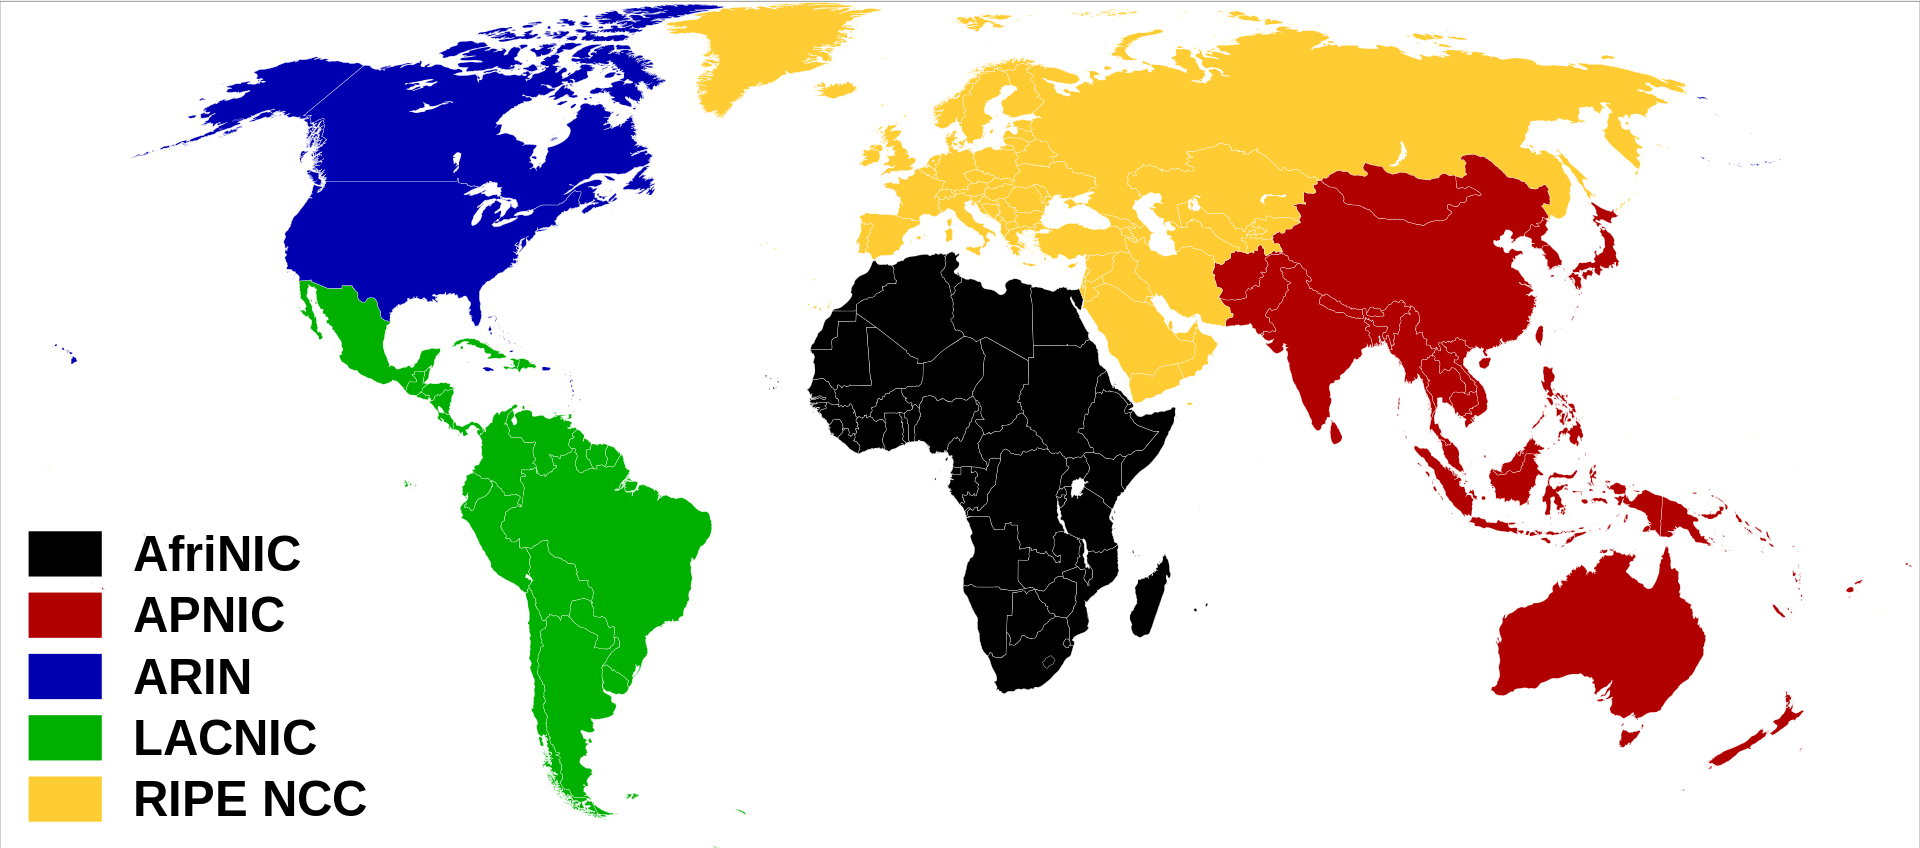
\includegraphics[width=\linewidth]{images/rirs.png}
  \caption{Regional Internet Registries manage the IP block assignment and Autonomous Systsem Number assignment for geographically local areas.}
  \label{fig:rirs}
\end{figure}
Before understanding the weaknesses of Internet routing, one must understand how the Internet routing system is intended to work.  Organizations rely on Internet Service Providers (ISPs) to direct their network traffic to the appropriate destinations.  Any organization that wants to connect to the Internet must be loaned an IP address from an ISP or assigned a block of IP addresses from a \emph{Regional Internet Registry (RIR)}.  RIRs manage IP address alloation for regions around the world, and Figure \ref{fig:rirs} shows examples of RIRs and their associated regions.  As depicted in Figure \ref{fig:rir-assignments}, organizations that are assigned IP addresses by an RIR must also be assigned an \emph{Autonomous System Number (ASN)}.  ASNs are unique numbers which identify an organization's network in the global Internet.

\begin{figure}[ht]
  \begin{center}
    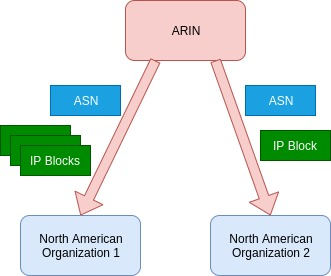
\includegraphics[width=0.6\linewidth]{images/rir-assignments.jpg}
  \end{center}
  \caption{Regional Internet Registries often assign a single ASN for each organization.  They also often assign one or many contiguous IP blocks to those organizations.}
  \label{fig:rir-assignments}
\end{figure}

\begin{figure}[hb]
  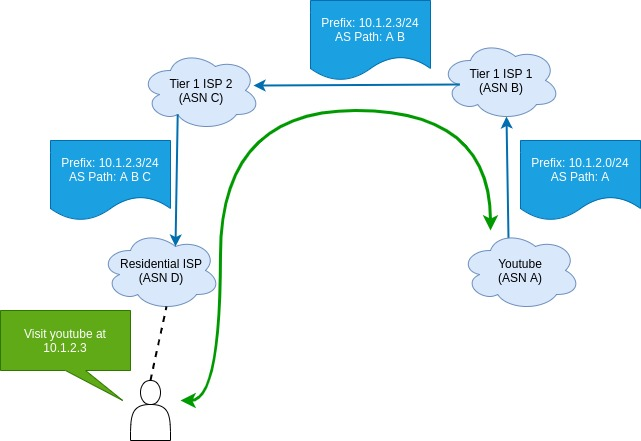
\includegraphics[width=\linewidth]{images/bgp-ops.jpg}
  \caption{The Border Gateway Protocol is used to announce the source of IP prefixes into the global Internet and to create paths from other organization's networks to those IP addresses.  The blue path represents the flow of BGP announcements for the Youtube IP prefix, and the green path represents the user's actual Youtube traffic.}
  \label{fig:bgp-ops}
\end{figure}

\section{Internet Routing Operation}
In order to reach services like Youtube, users must be provided with a network path to reach the service.  Youtube may have a set of IP addresses for users to connect, but there are still two challenges:
\begin{enumerate}
 \item Youtube needs to announce where those IP addresses exist in the Internet
 \item The Internet must find paths to reach Youtube
\end{enumerate}
The \emph{Border Gateway Protocol (BGP)} is used to solve these problems, as illustrated in Figure \ref{fig:bgp-ops}.  Continuing with the Youtube example, Youtube announces its addresses as an IP prefix\footnote{An IP prefix could be one of the blocks assigned to the organization, or it could be a contiguous subset of IP addresses within that block.} into its ISP, which resolves challenge 1.

In that same announcement, Youtube also announces its ASN.  When Youtube's ISP connects to another network, it appends its own ASN after Youtube's ASN to make an ordered list that describes a path.  This process continues throughout the Internet, allowing for each network to know which paths it can take to reach Youtube.  These paths, known as \emph{AS paths}, all begin with Youtube's ASN, which maps Youtube's ASN to its IP space in the global Internet.  These AS paths are used to address challenge 2.

If there are multiple paths to a target IP address, BGP uses a multi-step decision process to determine which route is preferred\footnote{The BGP decision process is not standardized, and it may vary across different implementations.  Many implementations are very similar.}.  The route with the shortest AS path length for a given destination is often the preferred route.

\section{BGP Hijacking}
With an understanding of how BGP operates, it is helpful to revisit the Youtube outage previously introduced.  Pakistan's state-run network had attempted to take all traffic in its network destined for Youtube's IP prefixes and drop it.  By mistake, this change in their internal network was announced to the rest of the Internet via BGP.  Figure {fig:bgp-hijack} illustrates what may have happened for some users who experienced a Youtube outage.  This was an example of \emph{BGP hijacking}, and it highlights a weakness in BGP: the receiver of the BGP announcement trusts the sender of the announcement, who trusted the sender of the previous BGP announcement, and so on.  This trust model is known as \emph{transitive trust}, and it is part of why BGP is not secure.  BGP hijacking can be unintentional, such as the Youtube example, but it can also be intentionally performed by malicious actors for data interception, eavesdropping, or denial of service.  Both intentional and unintentional BGP hijacking occur on a near-daily basis\cite{b1}.

\begin{figure}[ht]
  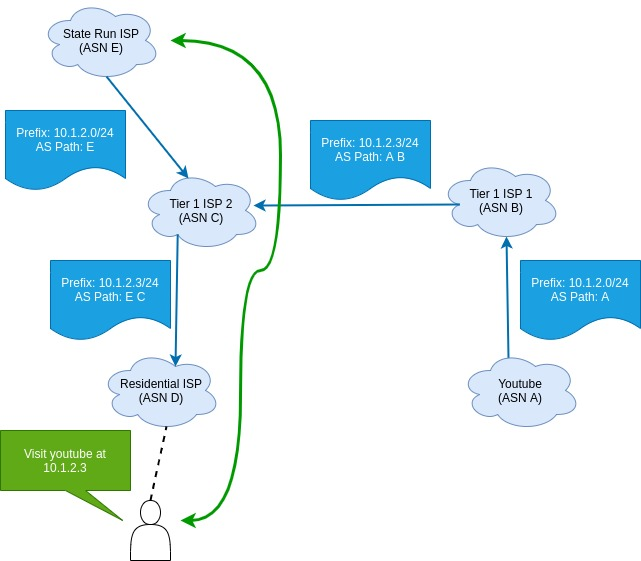
\includegraphics[width=\linewidth]{images/bgp-hijack.jpg}
  \caption{The state run network of Pakistan announced ownership of Youtube's IP prefixes to the rest of the world.  For many users, this ended up being the shortest AS path between them and Youtube.  The blue path represents the flow of BGP announcements for the Youtube IP prefix, and the green path represents the user's actual Youtube traffic.}
  \label{fig:bgp-hijack}
\end{figure}

\section{BGP Hijacking Mitigation Techniques}
Multiple techniques exist to address BGP hijacking, each with varying effectiveness and cost.  Three such techniques are \emph{Filtering}, \emph{Resource Public Key Infrastructure (RPKI)}, and \emph{BGPsec}.  Filtering has been used for a number of years, while RPKI and BGPsec are only recently seeing adoption.  A brief comparison of these techniques is presented in Table \ref{tab:bgp-hijacking-comparison} at the end of this chapter.

\subsection{Filtering}
Filtering is a technique to prevent propagating incorrect announcements from neighbors.  There are numerous BGP filtering methods, with two examples being AS path filtering and IP prefix filtering.  AS path filtering only allows a set of whitelisted ASNs to be accepted in BGP announcements.  This is effective for ISPs near the edge of the Internet, as those ISPs can choose to only accept AS paths comprised of the organization's ASN\footnote{Organizations can similarly apply AS path filtering on egress of their announcements to avoid accidental propagation of incorrect ASNs}.  IP prefix filtering is similar to AS path filtering, only it is applied to specific whitelisted IP prefixes.  Given that BGP hijacking events are still relatively frequent, filtering alone appears insufficient to prevent BGP hijacking.

\subsection{Resource Public Key Infrastructure for Origin Validation}
As noted previously, RIRs have a central mapping of IP prefixes to ASNs, and the first ASN in an AS path should correspond to the associated IP prefix in an announcement.  The mapping of ASNs to IP prefixes be used to validate the origin of BGP announcements.  This approach is used by operators who uncover BGP hijacking events after they have occurred, and it is also the concept behind Resource Public Key Infrastructure (RPKI).  RPKI automates origin validation by having the RIRs host digitally signed information, known as \emph{Route Organization Authorizations (ROAs)} confirming that an AS has authority to originate an IP prefix.  RPKI implementations vary by RIR, but one example is presented in Figure \ref{fig:rpki-assignment}.  Figure \ref{fig:rpki-ops} shows RPKI origin validation in action.

\begin{figure}[hp]
  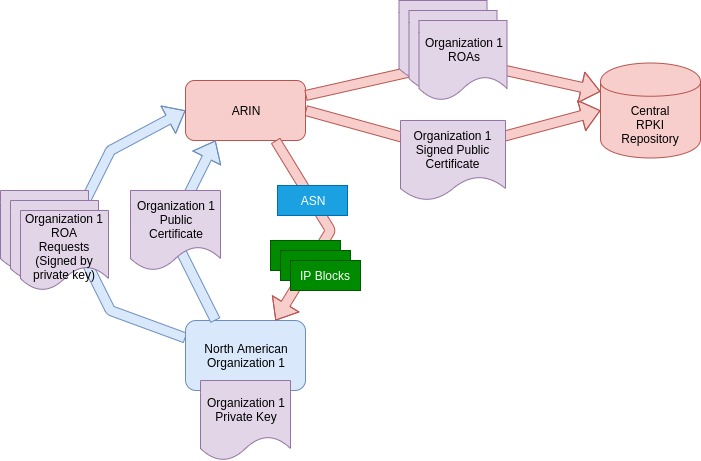
\includegraphics[width=\linewidth]{images/rir-rpki-assignments.jpg}
  \caption{This is an example of how ARIN implements RPKI.  The organization is assigned an ASN and a set of IP blocks.  If the organization participates in RPKI, then it generates a private key and a public certificate.  It sends the public certificate to be signed by the RIR.  The organization also generates ROA requests for its ASN and IP blocks, and it signs the request with its private key.  If ARIN deems the ROA request valid, then it generates an ROA and places it in the ROA database, where it can be used to validate the origin of BGP prefixes.}
  \label{fig:rpki-assignment}
\end{figure}

\begin{figure}[hp]
  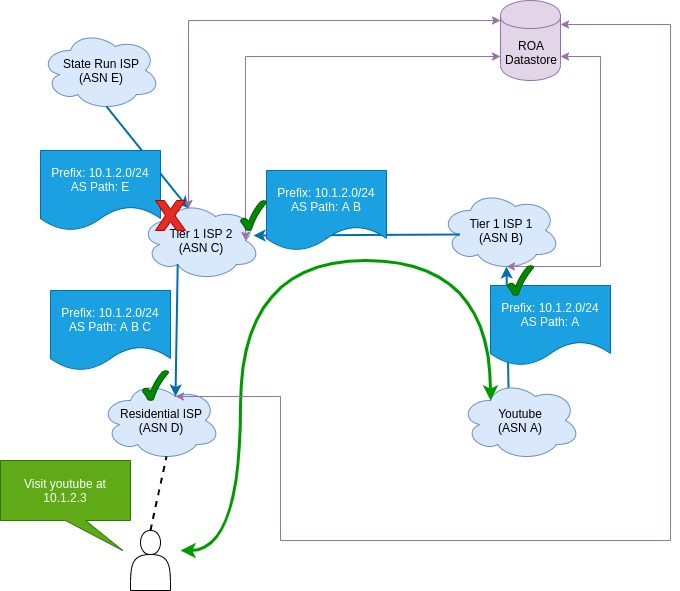
\includegraphics[width=\linewidth]{images/rpki-ops.jpg}
  \caption{If RPKI origin validation is in use, then routers can verify each BGP announcement by verifying that the first ASN in the AS path matches the origin of the IP prefix in the ROA database.  If there is a match, then the announcement is accepted and the associated routes may be propagated through the Internet.  If there is no match, then the route in the advertisement can be rejected.}
  \label{fig:rpki-ops}
\end{figure}

\begin{figure}[hp]
  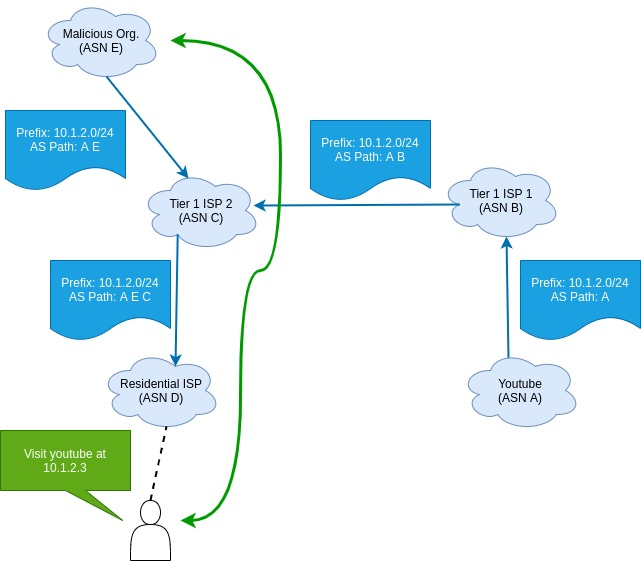
\includegraphics[width=\linewidth]{images/bgp-intercept.jpg}
  \caption{A malicious actor could announce a bogus route for a prefix with an AS path that includes the correct originating ASN and the malicious organization's ASN in the middle.  The malicious organization could choose to either terminate the connection by doing something like hosting a fake version of Youtube, or they could pass the traffic along to the real Youtube and capture the traffic passing through for offline analysis.  If this information includes encrypted financial information such as bank account numbers, then offline analysis could return highly valuable information.}
  \label{fig:bgp-intercept}
\end{figure}

\begin{figure}[hp]
  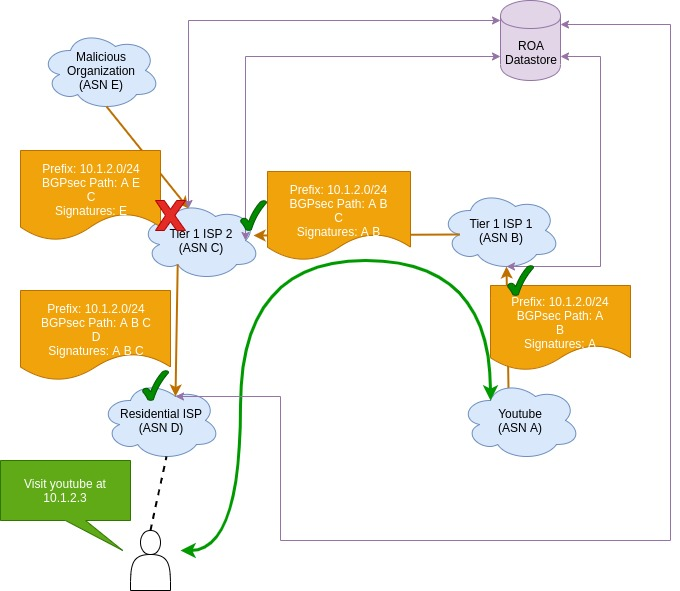
\includegraphics[width=\linewidth]{images/bgpsec-ops.jpg}
  \caption{If BGPsec is in use, then routers can verify each BGP announcement by verifying that each ASN in the BGPsec path has signatures which match the ROA database.  If each ASN in the path has valid signaturse, then the announcement is accepted and the associated routes may be propagated through the Internet.  If any single ASN in the path does not match, or if the origin ASN does not own the advertised prefix according to the ROA database, then the route in the advertisement can be rejected.}
  \label{fig:bgpsec-ops}
\end{figure}

\subsection{BGPsec}
RPKI prevents many cases of BGP hijacking, but it doesn't resolve all of them.  Consider malicious actors who want to intercept data destined for Youtube.  RPKI can detect a malicious network announcing it owns the Youtube IP space, but it cannot detect the case in Figure \ref{fig:bgp-intercept} of a malicious network announcing a path that passes through but does not originate from the malicious network, even if that path is fake.

A protocol known as BGPsec attempts to prevent this case by leveraging the RPKI infrastructure for full path validation.  BGPsec replaces the AS path with a \emph{BGPsec path} and places requirements on how the path can be modified.  The AS constructing the announcement can only provide its own ASN and the ASN of the BGPsec announcment recipient.  The AS constructing the announcement must provide a signature using the organization's RPKI private key.  As shown in Figure \ref{fig:bgpsec-ops}, recipients of a BGPsec announcement can validate the chain of ASNs in the BGPsec path by checking the associated signatures against the ROA database.

\section{Conclusion}
This chapter illustrated the key weakness of transitive trust in the Internet routing protocol known as BGP, and it showed how this weakness can be exploited through BGP hijacking.  Filtering, RPKI, and BGPsec were introduced as techniques for addressing BGP hijacking.

\begin{thebibliography}{00}
\bibitem{b1} https://www.noction.com/blog/bgp-hijacking
\end{thebibliography}

\newpage

\begin{table*}
\caption{Comparison of BGP Hijacking Mitigation Methods}
\label{tab:bgp-hijacking-comparison}
\begin{tabular}{|l|l|l|}
\hline
\textbf{Approach} & \textbf{Benefits}                                                                                                                                                      & \textbf{Drawbacks}                                                                                                                                                                                                                                   \\ \hline
Filtering         & \begin{tabular}[c]{@{}l@{}} \textbullet Widely available\\ \textbullet Computationally inexpensive\\ \textbullet No coordination needed to set up\end{tabular}                                        & \begin{tabular}[c]{@{}l@{}} \textbullet Can only be applied in certain cases near edge\\ \textbullet Configuration is rigid\\ \textbullet Empirically shown to be insufficient\\   (near-daily   hijacking incidents)\end{tabular}                                                        \\ \hline
RPKI              & \begin{tabular}[c]{@{}l@{}} \textbullet Mitigates many cases; would have prevented\\   Youtube/Pakistan incident\\ \textbullet Can be added on to existing Internet routing system\end{tabular} & \begin{tabular}[c]{@{}l@{}} \textbullet Moderately more computationally expensive\\ \textbullet Can delay valid routing changes compared\\   to unsecured BGP\\ \textbullet Requires additional backend setup and configuration\\ \textbullet Does not prevent malicious actors case\end{tabular} \\ \hline
BGPsec            & \begin{tabular}[c]{@{}l@{}} \textbullet Can mitigate all presented weaknesses;\\   prevents malicious actors case\\ \textbullet Explicitly breaks transitive trust model\end{tabular}           & \begin{tabular}[c]{@{}l@{}} \textbullet Requires replacing entire Internet routing system\\   for fully secure operation\\ \textbullet Significantly more computationally expensive\\ \textbullet Can delay valid routing changes compared\\   to unsecured BGP\end{tabular}                \\ \hline
\end{tabular}
\end{table*}
\end{document}
